%\documentclass{article}
%\usepackage{tikz,pgfplots}
%\usepackage[pdftex,active,tightpage]{preview}
%\begin{document}
%\begin{preview}
%%%%%%%%%%%%%%%%%%%%%%%%%%%%%%
%\pgfplotsset{every axis plot/.append style={very thick}}
%\begin{tikzpicture}%[scale=1/.618]
%%\node at (1,1) {asdf};%
%\begin{axis}[%
%	%grid=both,%
%	%xmajorgrids,%
%	xtick=data,%
%	xticklabels={T,S,R,Q,P,O,N,M,L,K,J,I,H,G,F,E,D,C,B},%
%	title={linearly spaced (1:19)},
%]
%% Line plot
%\addplot
%	plot [ only marks,
%	      	error bars/.cd,
%	      	y dir=both,y explicit ]
%	coordinates{
%	(1 ,0.0013) +- (0,0.0169)   %T
%	(2 ,0.3200) +- (0,0.0852)   %S
%	(3 ,0.3700) +- (0,0.0386)   %R
%	(4 ,0.2541) +- (0,0.0376)   %Q
%	(5 ,0.5624) +- (0,0.0524)   %P
%	(6 ,0.4278) +- (0,0.0778)   %O
%	(7 ,0.4997) +- (0,0.1010)   %N 6555
%	(8 ,0.5473) +- (0,0.0404)   %M 6555
%	(9 ,0.6198) +- (0,0.0696)   %L
%	(10,0.4236) +- (0,0.1020)   %K
%	(11,0.6262) +- (0,0.1148)   %J
%	(12,0.6038) +- (0,0.0589)   %I
%	(13,0.7312) +- (0,0.0598)  %H
%	(14,0.5873) +- (0,0.0856)   %G
%	(15,0.6347) +- (0,0.0960)  %F
%	(16,0.7222) +- (0,0.0316)  %E
%	(17,0.8714) +- (0,0.0174)  %D
%	(18,0.7733) +- (0,0.0389)  %C
%	(19,1.0000) +- (0,0.0000)  %B
%};
%\pgfplotsset{every axis legend/.append style={at={(0.618,0.2)},anchor=base}}
%\legend{$E_{norm}$}
%\end{axis}
%\end{tikzpicture}
%%%%%%%%%%%%%%%%%%%%%%%%%%%%%%
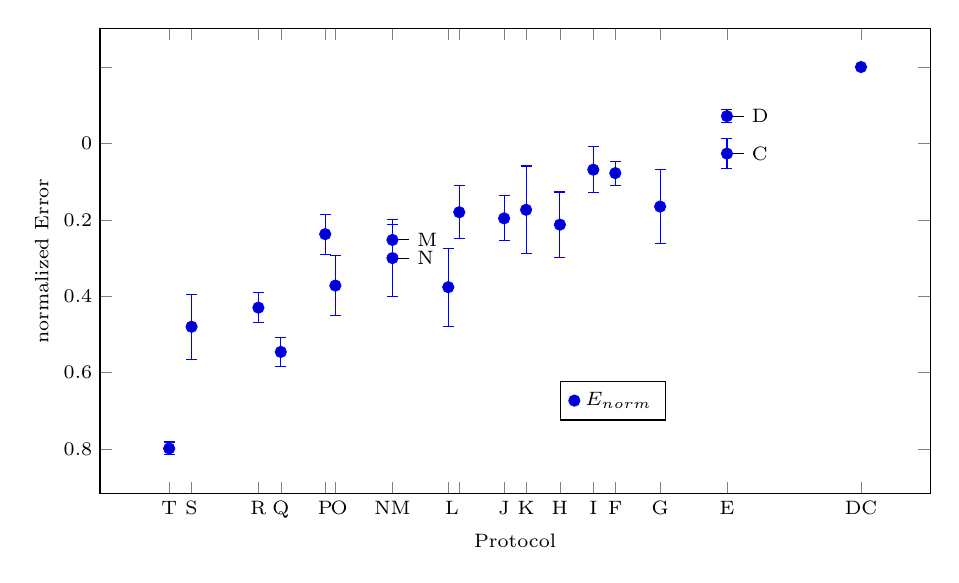
\begin{tikzpicture}%[scale=1/.618]
%\node at (1,1) {asdf};%
\begin{axis}[%
	width=\linewidth,
	height=0.618\linewidth,
	%grid=both,%
	%xmajorgrids,%
	xtick=data,%
	xticklabels={T,S,R,Q,P\ ,\ O,NM,,\ L,K\ ,J,I,H,G,F,E,DC,,B},%
	yticklabels={1,0.8,0.6,0.4,0.2,0},
	%title={spaced with total \#Projections (2185:15732)},%
	xlabel={Protocol},%
	ylabel={normalized Error}%
]
% Line plot
\addplot
	plot [ only marks,
	      	error bars/.cd,
	      	y dir=both,y explicit ]
	coordinates{
	(2.64,0.0013)  +- (0,0.0169) %T  2185
	(3.17,0.3200)  +- (0,0.0852) %S  2622
	(4.75,0.3700)  +- (0,0.0386) %R  3933
	(5.28,0.2541)  +- (0,0.0376) %Q  4370
	(6.33,0.5624)  +- (0,0.0524) %P  5244
	(6.57,0.4278)  +- (0,0.0778) %O  5436
	(7.92,0.4997)  +- (0,0.1010) %N  6555
	(7.92,0.5473)  +- (0,0.0404) %M  6555
	(9.5,0.6198)   +- (0,0.0696) %L  7866
	(9.24,0.4236)  +- (0,0.1020) %K  7648
	(11.08,0.6262) +- (0,0.1148) %J  9177
	(10.56,0.6038) +- (0,0.0589) %I  8740
	(12.67,0.7312) +- (0,0.0598) %H 10488
	(11.88,0.5873) +- (0,0.0856) %G  9833
	(14.25,0.6347) +- (0,0.0960) %F 11799
	(13.19,0.7222) +- (0,0.0316) %E 10925
	(15.83,0.8714) +- (0,0.0174) %D 13110
	(15.83,0.7733) +- (0,0.0389) %C 13110
	(19,1.0000)    +- (0,0.0000) %B 15732
};
\pgfplotsset{every axis legend/.append style={at={(0.618,0.2)},anchor=base}}
\legend{$E_{norm}$}

\tikzstyle{every pin}=[font=\footnotesize]

%\node [coordinate,pin=below right:C] at (axis cs:15.83,0.7733) {};
%\node [coordinate,pin=above right:D] at (axis cs:15.83,0.8714) {};
%\node [coordinate,pin=above right:M] at (axis cs:7.92 ,0.5773) {};
%\node [coordinate,pin=below right:N] at (axis cs:7.92 ,0.4997) {};

\scriptsize
\draw [] (axis cs:15.83,0.7733) -- (axis cs:16.23,0.7733) node [right] {C};
\draw [] (axis cs:15.83,0.8714) -- (axis cs:16.23,0.8714) node [right] {D};
\draw [] (axis cs:7.92,0.5473) -- (axis cs:8.32,0.5473) node [right] {M};
\draw [] (axis cs:7.92,0.4997) -- (axis cs:8.32,0.4997) node [right] {N};

\end{axis}

\end{tikzpicture}
%%%%%%%%%%%%%%%%%%%%%%%%%%%%%%
% plot erstellt mit MATLAB-File p:\doc\MATLAB\WFS-CompareDMPs\wfs_Compare2008c.m (FromToTo = 1:5:1024)
% und matlab2tikz
% Daten
% neue Version
%>> [ 1:19;mean(fliplr(max(max(NormCumulativeError))-NormCumulativeError));std(fliplr(NormCumulativeError))]
%
%ans =
%
%  Columns 1 through 12
%
%    1.0000    2.0000    3.0000    4.0000    5.0000    6.0000    7.0000    8.0000    9.0000   10.0000   11.0000   12.0000
%    0.0013    0.3200    0.3700    0.2541    0.5624    0.4278    0.4997    0.5473    0.6198    0.4236    0.6262    0.6038
%    0.0169    0.0852    0.0386    0.0376    0.0524    0.0778    0.1010    0.0404    0.0696    0.1020    0.1148    0.0589
%
%  Columns 13 through 19
%
%   13.0000   14.0000   15.0000   16.0000   17.0000   18.0000   19.0000
%    0.7312    0.5873    0.6347    0.7222    0.8714    0.7733    1.0000
%    0.0598    0.0856    0.0960    0.0316    0.0174    0.0389         0
% Alte, falsch ausgerichtete Version
%[ 1:19;std(NormCumulativeError);mean(NormCumulativeError)]
%
%ans =
%
%  Columns 1 through 12
%
%    1.0000    2.0000    3.0000    4.0000    5.0000    6.0000    7.0000    8.0000    9.0000   10.0000   11.0000   12.0000
%         0    0.0389    0.0174    0.0316    0.0960    0.0856    0.0598    0.0589    0.1148    0.1020    0.0696    0.0404
%         0    0.2267    0.1286    0.2778    0.3653    0.4127    0.2688    0.3962    0.3738    0.5764    0.3802    0.4527
%
%  Columns 13 through 19
%
%   13.0000   14.0000   15.0000   16.0000   17.0000   18.0000   19.0000
%    0.1010    0.0778    0.0524    0.0376    0.0386    0.0852    0.0169
%    0.5003    0.5722    0.4376    0.7459    0.6300    0.6800    0.9987          	
%%%%%%%%%%%%%%%%%%%%%%%%%%%%%%
%\end{preview}
%\end{document}